\documentclass[conference, 11pt]{IEEEtran}
\usepackage{graphicx}
\usepackage[utf8x]{inputenc}
\usepackage{longtable}
\usepackage[T1]{fontenc}
\usepackage{amsmath}
\usepackage{color}
\usepackage{caption}
\definecolor{dkgreen}{rgb}{0,0.6,0}
\definecolor{gray}{rgb}{0.5,0.5,0.5}
\definecolor{mauve}{rgb}{0.58,0,0.82}
\DeclareCaptionFont{white}{\color{white}}
\DeclareCaptionFormat{listing}{\colorbox{gray}{\parbox{\linewidth}{#1#2#3}}}
\captionsetup[lstlisting]{format=listing,labelfont=white,textfont=white}
\usepackage{listings}
\lstset{ %
  basicstyle=\footnotesize,           % the size of the fonts that are used for the code
  numbers=left,                   % where to put the line-numbers
  numberstyle=\tiny\color{gray},  % the style that is used for the line-numbers
  stepnumber=1,                   % the step between two line-numbers. If it's 1, each line 
                                  % will be numbered
  numbersep=5pt,                  % how far the line-numbers are from the code
  backgroundcolor=\color{white},      % choose the background color. You must add \usepackage{color}
  showspaces=false,               % show spaces adding particular underscores
  showstringspaces=false,         % underline spaces within strings
  showtabs=false,                 % show tabs within strings adding particular underscores
  %frame=single,                   % adds a frame around the code
  rulecolor=\color{black},        % if not set, the frame-color may be changed on line-breaks within not-black text (e.g. commens (green here))
  tabsize=2,                      % sets default tabsize to 2 spaces
  captionpos=t,                   % sets the caption-position to bottom
  breaklines=true,                % sets automatic line breaking
  breakatwhitespace=false,        % sets if automatic breaks should only happen at whitespace
  title=\lstname,                   % show the filename of files included with \lstinputlisting;
                                  % also try caption instead of title
  keywordstyle=\color{blue},          % keyword style
  commentstyle=\color{dkgreen},       % comment style
  stringstyle=\color{mauve},         % string literal style
  escapeinside={\%*}{*)},            % if you want to add a comment within your code
  morekeywords={*,...}               % if you want to add more keywords to the set
}



\begin{document}

\title{SecureIt: home security\\
via Android application}

\author{
\IEEEauthorblockN{Luca Bonato, Marco Ziccardi}
\IEEEauthorblockA{Corso di studi in Informatica\\
Università degli Studi di Padova\\
Email: \{lohathe,marco.ziccard\}@gmail.com}
}


\maketitle


\begin{abstract}
Nowadays different applications offer a mechanism to monitor your home in order to detect any intrusion. Nevertheless none of these solutions completely exploits phone functionalities to find intruders: accelerometer, camera or microphone are often mutually exclusive. Moreover none of these applications tracks phone's position after an intrusion has been identified. The proposed application aims to collect different solution for motion/presence detection and to track phone's position using any kind of connectivity.
\end{abstract}

\IEEEpeerreviewmaketitle

\section{\textbf{Introduction}}
Traditional surveillance systems rely on ad hoc and proprietary solutions and have weaknesses like poor mobility, high costs and low flexibility. Current smartphones spread makes possible to exploit these devices to protect our homes.\\

The developed application exploits phone's hardware in order to offer a traditional survellance system services.\\

The aim of the application development was not only the creation of a home security system but also the discovery of phone capabilities. 

\section{\textbf{Application overview}}
Operations performed by the application are complex and really resource needful:
\begin{itemize}
	\item Accelerometer to detect orientation and shake
	\item Camera to detect motion processing frames
	\item Microphone to detect environmental sound level
	\item Wifi or 3G connectivity to upload images and audio
	\item GPS to get current location
	\item Bluetooth to upload location in absence of connectivity
	\item In app encryption in order to securely authenticate the user
\end{itemize}

To the mobile application is associated a back-end where the application itself uploads images and audio got at the instant of the intrusion detection.\\

In order to allow the end user to select the type of monitoring and the type of alerting according to his needs about security, CPU and power consumption, a configuration panel (shown in figure \ref{img:config}) is presented at each start of the application.\\

\begin{figure}[!ht]
\begin{center}
\makebox[\linewidth]{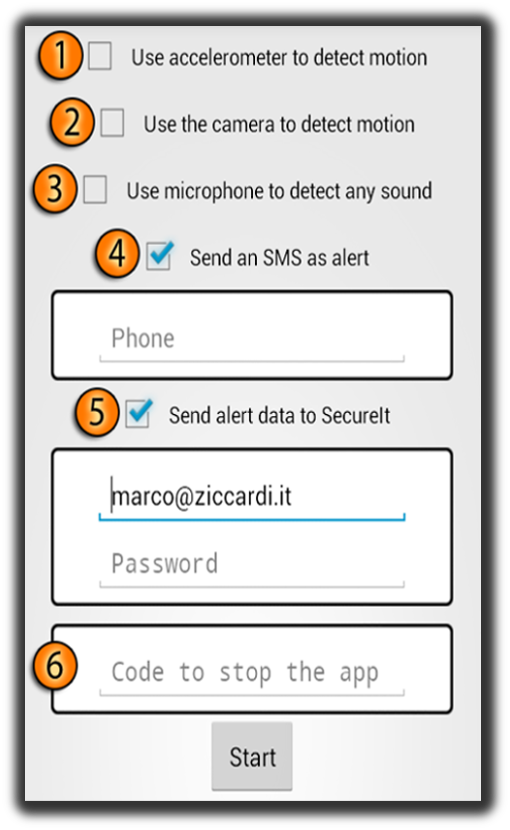
\includegraphics[scale=0.3]{resources/config.png}}
\caption{Configuration view}
\label{img:config}
\end{center}
\end{figure}

\begin{enumerate}
	\item Asks the application to use the accelerometer, shown only if the accelerometer is available on the phone
	\item Asks the application to use the camera, allows to choose which camera to use and to start the flash
	\item Asks the application to use the microphone
	\item Asks the application to send an SMS to the specified phone number to alert an intrusion
	\item Asks the application to authenticate and send images, audio and location to the back-end (images are sent only if camera has been activated). A username and a password have to be specified
	\item Allows to set the unlock code. Application can be closed only by writing that code
\end{enumerate}

\section{\textbf{Architecture}}

In figure \ref{img:architecture} is presented the developed application.

\begin{figure}[!ht]
\begin{center}
\makebox[\linewidth]{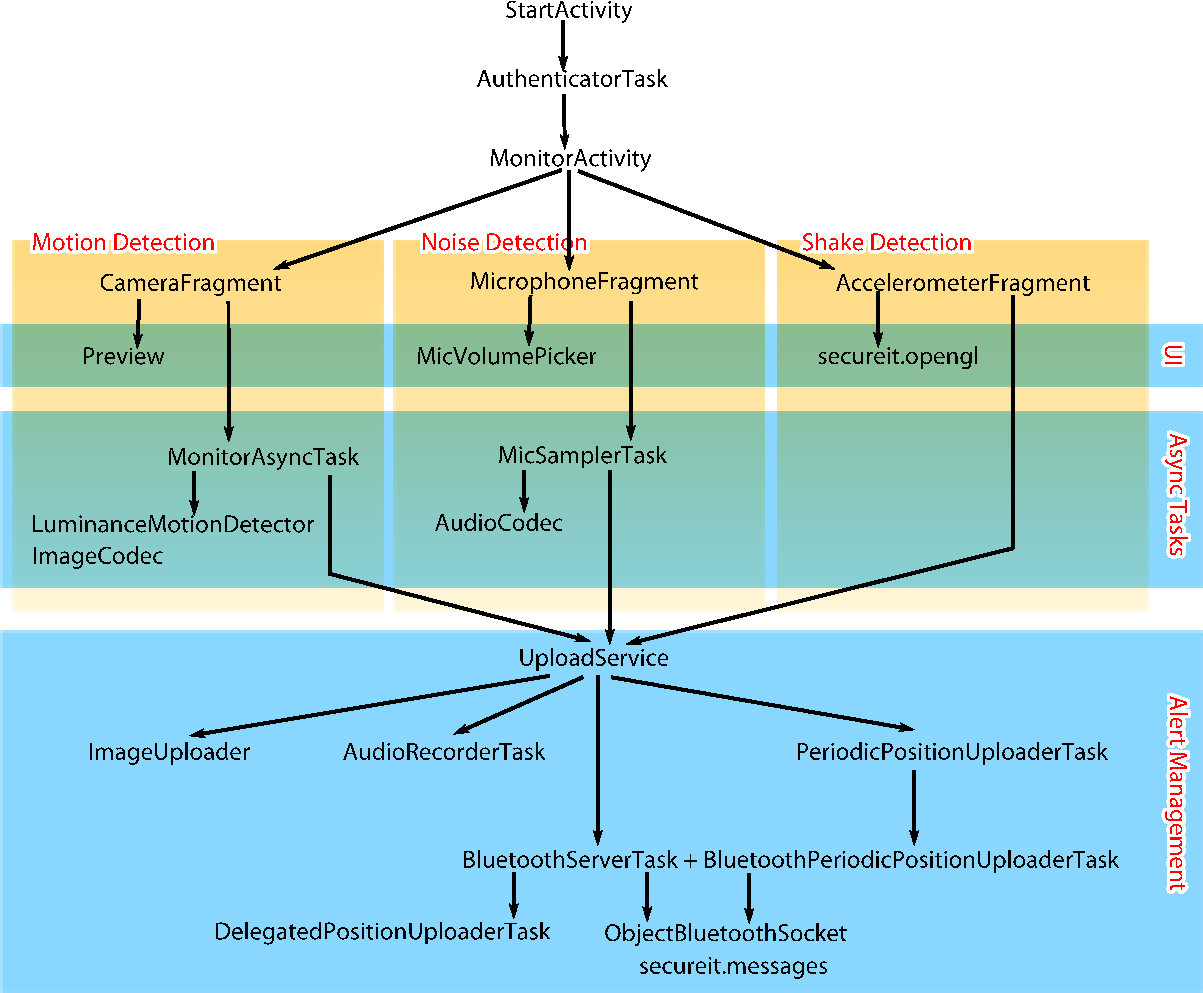
\includegraphics[scale=0.45]{resources/architecture.pdf}}
\caption{High level architecture diagram}
\label{img:architecture}
\end{center}
\end{figure}

Three parts can be identified which realize the monitoring tasks of the application. Each of that parts can be diveded in components:
\begin{itemize}
	\item \texttt{Motion Detection}:
		\begin{itemize}
			\item \texttt{CameraFragment}: active view component displayed by the Android \texttt{SDK}
			\item \texttt{Preview}: links camera hardware to the Java application
			\item \texttt{MonitorAsyncTask}: processes frames in order to detect motion
			\item \texttt{LuminanceMotionDetector}, \texttt{ImageCodec}: utility classes used by \texttt{MotionAsyncTask}
		\end{itemize}
	\item \texttt{Noise Detection}:
		\begin{itemize}
			\item \texttt{MicrophoneFragment}: active view component displayed by the Android \texttt{SDK}
			\item \texttt{MicVolumePicker}: passive view showing noise level
			\item \texttt{MicSamplerTask}: periodically samples audio data using \texttt{AudioCodec}
			\item \texttt{AudioCodec}: samples microphone on demand
		\end{itemize}
	\item \texttt{Motion Detection}:
		\begin{itemize}
			\item \texttt{AccelerometerFragment}: active view component displayed by the Android \texttt{SDK}
			\item \texttt{secureit.opengl}: package of view utilities to display 3D animations
		\end{itemize}
\end{itemize}

\texttt{UploadService} is activated by an alert coming from one of the framents presented before. It uses the following tasks to perform the data upload:
\begin{itemize}
	\item \texttt{ImageUploaderTask}: uploads the captured images
	\item \texttt{AudioRecorderTask}: records the audio and uploads it
	\item \texttt{PeriodicPositionUploaderTask}: periodically sends phone position to the back-end using \texttt{WIFI} or \texttt{3G} network
	\item \texttt{Bluetooth\allowbreak Periodic\allowbreak Position\allowbreak Uploader\allowbreak Task}: periodically sends phone position using opportunistic bluetooth connectivity, activated only if no \texttt{WIFI} or \texttt{3G} network is active
	\item \texttt{BluetoothServerTask}: task responding to bluetooth messages requesting delegated position upload
	\item \texttt{DelegatedPositionUploaderTask}: sends delegated phone position
\end{itemize}

Bluetooth message exchange is done using the following modules:

\begin{itemize}
	\item \texttt{ObjectBluetoothSocket}: object oriented socket for message delivery
	\item \texttt{secureit.messages}: package containing bluetooth messages
\end{itemize}


\section{\textbf{Intrusion detection}}
Intrusion detection is performed through three complementary ways:
\begin{itemize}
	\item \textbf{Accelerometer}
	\item \textbf{Camera}
	\item \textbf{Microphone}
\end{itemize}

\subsection{\textbf{Accelerometer}}
The accelerometer is used to detect motion of the phone itself. Different sensitivity can be set in order to detect different kinds of motions.\\
The accelerometer returns a \textit{triple} of three acceleration values on the three axes (\textit{X}, \textit{Y} and \textit{Z}). 

\begin{figure}[!ht]
\begin{center}
\makebox[\linewidth]{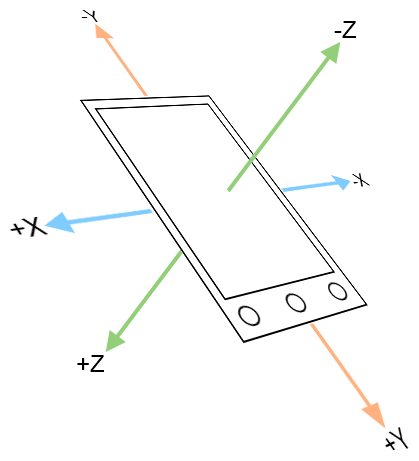
\includegraphics[scale=0.6]{resources/accelerometer.png}}
\caption{Values and signs of detected acceleration}
\end{center}
\end{figure}

Those values allow to detect every orientation taken by the phone except for phone rotations on the \textit{Z} axis when the phone is vertical (this is obvious according to the fact that in such a position the phone is not subject to acceleration variations on that axis).\\
Those acceleration values are used to move a 3D animation made in OpenGL ES (running on the GPU) that simply uses them to show phone's orientation, see figure \ref{img:opengl}.

\begin{figure}[!ht]
\begin{center}
\makebox[\linewidth]{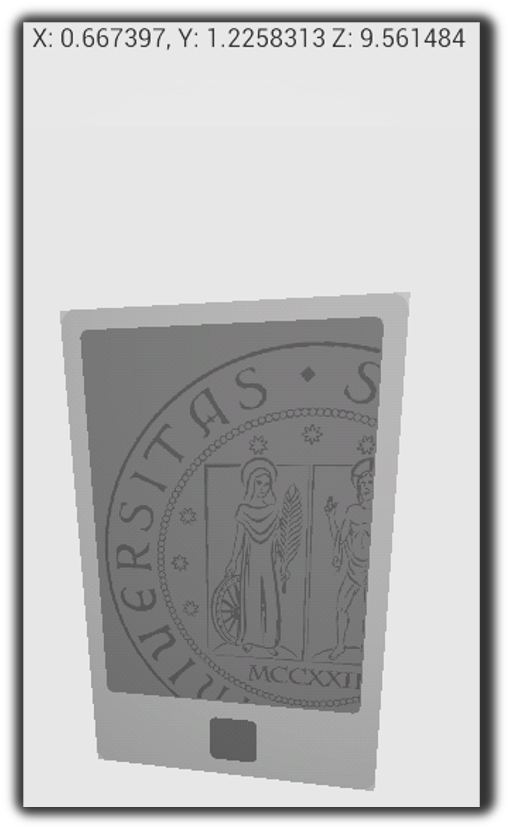
\includegraphics[scale=0.3]{resources/opengl.png}}
\caption{OpenGL ES 3D animation to show phone orientation}
\label{img:opengl}
\end{center}
\end{figure}


Acceleration triple is also used to detect any variation in the phone acceleration. Acceleration variation gives an idea of intensity of phone's \textit{shake} and it is computed as in equation \ref{eq:accel_variation}.

\begin{equation}
variation = \frac{(\Delta accelX)+(\Delta accelY)+(\Delta accelZ)}{\Delta t}
\label{eq:accel_variation}
\end{equation}\\
Three levels of sensitivity are defined:
\begin{itemize}
	\item \texttt{LOW}: \texttt{SHAKE\_THRESHOLD = 3100}
	\item \texttt{MEDUM}:  \texttt{SHAKE\_THRESHOLD = 2700}
	\item \texttt{HIGH}:  \texttt{SHAKE\_THRESHOLD = 2300}
\end{itemize}

If $variation>\texttt{SHAKE\_THRESHOLD}$ the application starts to send alerts according to the specified options.

\subsection{\textbf{Camera}}
The camera is used to detect motion in the surrounding environment. The frames captured by the camera are processed to detect if any variation has occurred since the previous captured frame.\\
A callback is activated at every captured frame; processing each captured frame would be too expensive for the phone in terms of CPU usage and battery consumption, processing is therefore reduced at one frame per second.\\
\subsubsection{\textbf{Motion detection}}
As said motion detection on the frame matrix is very expensive so the frames are scaled as soon as capture to a size of \texttt{640x480}. In order to detect any variation between two frames only the gray-scale image is needed.\\
A movement is considered to be a difference in number of pixels between two gray-scale frames bigger than a certain threshold.\\
Also in that case we have three types of sensitivity, the sensitivity type defines not only the threshold in the number of different pixels (\texttt{NUMBER\_THRESHOLD}) but also the threshold needed to consider different two pixels (\texttt{VALUE\_THRESHOLD}):

\begin{itemize}
	\item \texttt{LOW}:
		\begin{itemize}
		\item \texttt{VALUE\_THRESHOLD = 60}
		\item \texttt{NUMBER\_THRESHOLD = 20000}
		\end{itemize}
	\item \texttt{MEDUM}:
		\begin{itemize}
		\item \texttt{VALUE\_THRESHOLD = 50}
		\item \texttt{NUMBER\_THRESHOLD = 10000}
		\end{itemize}
	\item \texttt{HIGH}:
		\begin{itemize}
		\item \texttt{VALUE\_THRESHOLD = 40}
		\item \texttt{NUMBER\_THRESHOLD = 9000}
		\end{itemize}
\end{itemize}

Supposing to represent the two frames to compare with two linearized arrays of integer representing each pixel value the pseudo-code used form motion detection is straightforward:

\begin{lstlisting}[language=Java, caption=Pseudocode for motion detection]
detectMotion(int[] oldImage,int[] newImage,int width,int height)
begin
	List differentPixels
	for (int i = 0, ij=0; i < height; i++){
		for (int j = 0; j < width; j++, ij++){
			int newPixelValue = newImage[ij]
			int oldPixelValue = oldImage[ij]
			if (|newPixelValue-oldPixelValue|>=VALUE_THRESHOLD){
	            differentPixels.add(ij);
			}
		}
	}
	return differentPixels		
end
\end{lstlisting}

The detection identifies the list of mutated pixels according to the sensitivity specified.\\

\subsubsection{\textbf{Data representation}}
In order to make the user understand what the application is doing a view is presented showing: the surface currently being captured by the camera, the last frame considered by motion detection and the current considered frame; pixel identified as changed are marked in red in the current frame. This view is shown in figure \ref{img:camera}.

\begin{figure}[!ht]
\begin{center}
\makebox[\linewidth]{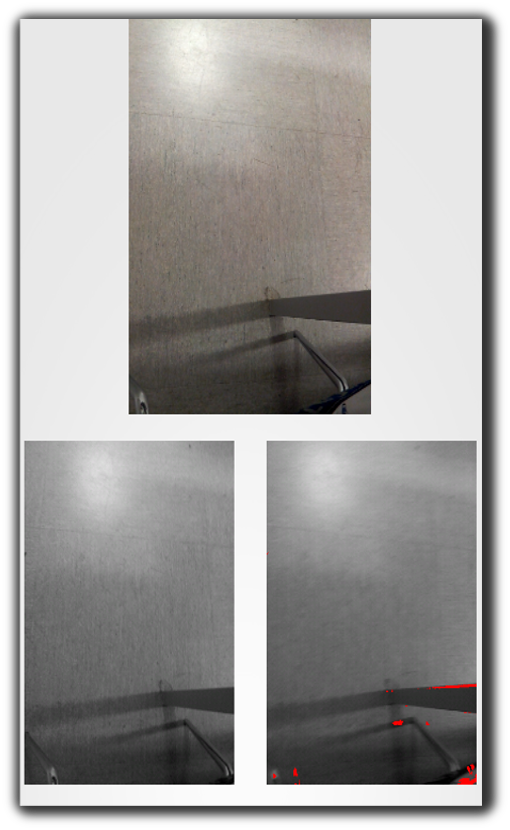
\includegraphics[scale=0.3]{resources/camera.png}}
\caption{Camera view to show motion detected}
\label{img:camera}
\end{center}
\end{figure}

\subsection{\textbf{Microphone}}
The microphone is used to detect an excessive noise level in the environment. In that case too three levels of sensitivity are defined each of one refers to a different value of decibels.

\begin{itemize}
	\item \texttt{LOW}: \texttt{NOISE\_THRESHOLD = 60}
	\item \texttt{MEDUM}:  \texttt{NOISE\_THRESHOLD = 50}
	\item \texttt{HIGH}:  \texttt{NOISE\_THRESHOLD = 30}
\end{itemize}~

\subsubsection{\textbf{Sampling}}
The application keeps sampling a buffer of \texttt{512} values of \texttt{16 BIT PCM}. Those values present the environment noise.\\ Scientific literature is plenty of tables showing for each common noise the corresponding decibel value, such as the one in figure \ref{img:decibels}. 

\begin{figure}[!ht]
\begin{center}
\makebox[\linewidth]{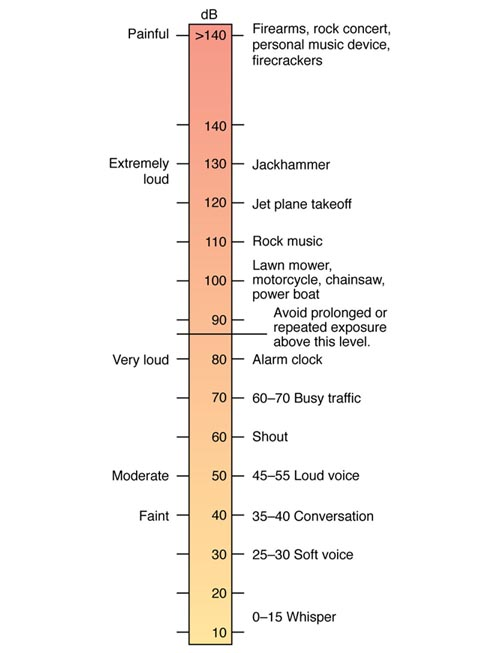
\includegraphics[scale=0.5]{resources/decibels.jpeg}}
\caption{A decibel scale}
\label{img:decibels}
\end{center}
\end{figure}

In order to exploit those tables and the user-friendliness of decibel \texttt{PCM} values are used to get \texttt{dB} values.\\ 
Referring to a measure of amplitude we can express the ratio of the squares between current value $V_i$ and a reference value $V_o$ in decibels as:

\begin{equation}
dB_i = 20log_{10} \left(\frac{V_i}{V_o}\right)
\end{equation}

To convert \texttt{PCM} values to \texttt{dB} we can suppose that each sampled value is different from \texttt{0} if the microphone samples something audible, so as a reference value to compute noise intensity from \texttt{PCM} the integer \texttt{1}, can be used.\\

Given the sample as an array (called \texttt{signal}) of \texttt{512 short integers} the following pseudo-code can be used to compute average \texttt{dB} intensity:

\begin{lstlisting}[language=Java, caption=Pseudocode for computing dB from PCM samples]
int total = 0
int count = 0
for (short peak : signal) {
	if (peak != 0) {
		total=total+|peak|
		count=count+1
	}
}
int average = 0
if (count > 0) average = total/count

double averageDB = 0.0
if (average!=0) {
	averageDB = 20*log10((average)/1)
}
\end{lstlisting}

\subsubsection{\textbf{Data representation}}

To make the end user aware of the ongoing process a view shows the decibels sampled by the microphones. The values are represented using a two channel volume indicator (in case of stereo microphones owned by some devices). Two levels are highlighted in the indicator: the first one is the threshold over which an alert is fired while the second one is an arbitrary noise threshold.

\begin{figure}[!ht]
\begin{center}
\makebox[\linewidth]{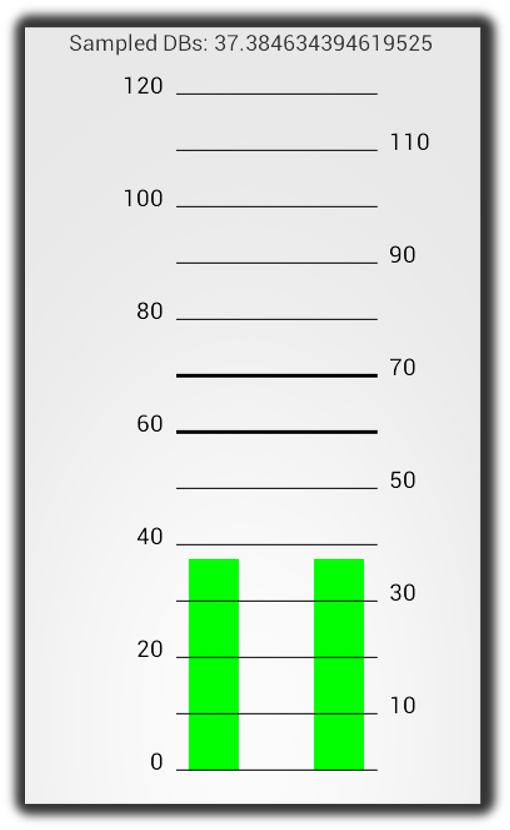
\includegraphics[scale=0.3]{resources/microphone.png}}
\caption{Microphone view to show sampled audio level}
\label{img:microphone}
\end{center}
\end{figure}

\section{\textbf{Alert communication}}
If a user is logged in, different ways of alert communication have been implemented depending on the connectivity currently available:
\begin{itemize}
	\item \texttt{WIFI CONNECTIVITY}: a set of 10 captured images and 10 seconds of audio are sent
	\item \texttt{3G CONNECTIVITY}: a subset of 5 captured images and 10 seconds of audio are sent
	\item \texttt{BLUETOOTH CONNECTIVITY}: no images or audio are sent but bluetooth is used to opportunistically and periodically request other devices to send phone's position
\end{itemize}

In both cases of \texttt{WIFI} or \texttt{3G CONNECTIVITY} a periodic task is used to send phone's location to the back-end.

\subsection{\textbf{Connectivity identification}}
In order to identify what kind of connectivity is available on the device the Android \texttt{APIs} are used. Those \texttt{APIs} allow to define whether the phone is connected or connecting. Confirmed that the phone is connected, the kind of connectivity is inspected via the following code:

\begin{lstlisting}[language=Java, caption=Java code to define connectivity type]
ConnectivityManager cm = (ConnectivityManager)
	getSystemService(Context.CONNECTIVITY_SERVICE);
boolean isConnected = false;
boolean isWifi = false;
NetworkInfo activeNetwork = 
	cm.getActiveNetworkInfo();
if (activeNetwork != null) {
	isConnected = 
		activeNetwork.isConnectedOrConnecting();
	isWifi = 
		activeNetwork.getType() == ConnectivityManager.TYPE_WIFI;
}
\end{lstlisting}

\subsection{\textbf{Authentication}}
A phone connected to \texttt{WIFI} or \texttt{3G} sends directly his data to the back-end, so it needs for sure an \texttt{access\_token}. Moreover a phone needs another type of token (for security purposes) in order to delegate via bluetooth other devices to send to the back-end his location. Such a token is called \texttt{delegated\_access\_token} and can be used by other devices to be authorized to post a location for the delegating phone.\\
A \texttt{REST API} (\texttt{[POST] /users/accesstoken}) can be used to get those tokens given username and password. The tokens are returned in the response body as \texttt{JSON}:

\begin{lstlisting}[language=Java, caption=Response body containing tokens]
{"access_token": "BASE64_TOKEN",
 "delegated_access_token": "BASE64_DELEGATED_TOKEN"}
\end{lstlisting}

\subsection{\textbf{Data upload}}
Images and audio are uploaded to the backend in a similar way. A \texttt{MULTIPART POST} request is sent to some \texttt{REST API} offered by the back-end, respectively:

\begin{lstlisting}[caption=REST API to upload images and audio]
[POST]	/api/phones/:phoneId/images
[POST] 	/api/phones/:phoneId/audio
\end{lstlisting}

For authentication purposes a request header field named \texttt{access\_token} is added.

\subsection{\textbf{Direct location upload}}
In case of \texttt{WIFI} or \texttt{3G CONNECTIVITY} location is directly uploaded by the phone. The \texttt{API} used is simply \texttt{[POST] /api/phones/:phoneid/positions} and the authentications still uses an \texttt{access\_token} header field.\\
Location data can be retrieved in two ways according to the phone capabilities:

\begin{itemize}
	\item \texttt{GPS}
	\item \texttt{NETWORK}
\end{itemize}

\section{\textbf{Bluetooth communication}}
As said when only bluetooth is active the phone asks other devices to upload his location. Two key features have been realized:

\begin{itemize}
	\item The communication is opportunistic, no need to pair devices
	\item Only authorized data is accepted
\end{itemize}

\subsection{\textbf{No pairing}}
Android offers two ways for creating a bluetooth server socket: \texttt{listen\allowbreak Using\allowbreak Rfcomm\allowbreak WithServiceRecord} and \texttt{listen\allowbreak Using\allowbreak Insecure\allowbreak RfcommWithServiceRecord}. The first method creates a server socket listening for incoming connections created via \texttt{create\allowbreak Rfcomm\allowbreak SocketToServiceRecord} and needs an explicit pairing of two devices with user acceptance. The second method instead allows to manage incoming connections that do not require pairing with user acceptance (created with \texttt{create\allowbreak Insecure\allowbreak Rfcomm\allowbreak SocketToServiceRecord}).\\

\subsection{\textbf{Delegated authorization}}
In the authentication phase a \texttt{delegated\allowbreak\_access\allowbreak\_token} is retrieved in order to not use the same token for both direct and delegated authentication. However such a token should not be shared with other devices and in order to do so a little protocol has been developed.\\
The protocol in figure \ref{img:bluetooth} is slightly inspired by Kerberos (\texttt{[1]}) and is based on three messages:\\

\begin{figure}[!ht]
\begin{center}
\makebox[\linewidth]{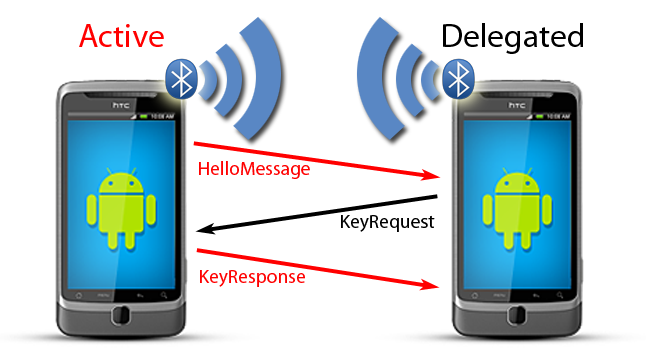
\includegraphics[scale=0.4]{resources/bluetooth.png}}
\caption{Bluetooth communication scheme}
\label{img:bluetooth}
\end{center}
\end{figure}

Each application running on a device with active bluetooth offers an insecure \texttt{RFCOMM} server socket able to accept insecure requests for a specified \texttt{UIID}.\\

When on any device running the application an intrusion is detected and no connectivity is available the bluetooth alert workflow starts:\\
\begin{enumerate}
	\item A bluetooth discovery is started
	\item A listener is registered to the process of discovery and each new device identified is stored
	\item As soon as discovery finishes the application tries to create a connection for each device, if it fails the device is discarded, otherwise a messaging workflow is started:
		\begin{enumerate}

			%Hello message
			\item An \texttt{HelloMessage} is sent. It contains a timestamp and the phone's identifier. \texttt{phoneId} is used by the delegated device to know who is requesting delegation, and where to upload location
			%Key request
			\item A \texttt{KeyRequest} is received. It is sent from the delegated device and contains latitude, longitude and a timestamp intended to be sent to the back-end
			%authorization_key creation
			\item An \texttt{authorization\_key} is computed via \texttt{AES} password encryption, using as password the value \texttt{delegated\_access\_token} and encrypting the \texttt{JSON} string reported in listing \ref{delegatedaccesstoken}.

\begin{lstlisting}[float, language=Java, caption=JSON encrypted with AES, label=delegatedaccesstoken]
{"lat": "latitude",
 "long": "longitude",
 "timestamp": "timestamp"}
\end{lstlisting}


			The code in listing \ref{encrypt} shows how to compute \texttt{AES} password encryption of the string in Java

\begin{lstlisting}[float, language=Java, caption=AES password encryption, label=encrypt]
SecretKeySpec key = new SecretKeySpec(password.getBytes(), "AES");
AlgorithmParameterSpec paramSpec = new IvParameterSpec(password.substring(0, 16).getBytes());
Cipher cipher;
cipher = Cipher.getInstance("AES/CBC/PKCS5Padding");	    
cipher.init(Cipher.ENCRYPT_MODE, key, paramSpec);			    	
byte[] ecrypted = cipher.doFinal(accessKey.getBytes());
accessKey = Base64.encodeToString(ecrypted, Base64.DEFAULT);
\end{lstlisting}	
			%Key response
			\item A \texttt{KeyResponse} is sent. It contains the \texttt{authorization\_key} that can be computed only by the requesting client since \texttt{delegated\_access\_token} is never shared
			%Data upload
			\item The delegated phone sends latitude, longitude, timestamp and \texttt{authorization\_key} to the \texttt{REST API [POST] /api\allowbreak/phones\allowbreak/:phoneid\allowbreak/position/delegated}
			%Authorization
			\item The back-end is able to decrypt \texttt{authorization\_key} using \texttt{delegated\_access\_token} of the requesting phone (\texttt{phoneId}) and verify that the owner has authorized the upload of latitude and longitude
		\end{enumerate}
	\item If location is sent correctly 1 hour is waited before next retransmission, otherwise only 1 minute is waited
\end{enumerate}

\subsection{\textbf{Android APIs improvement}}
Android \texttt{APIs} represent a bluetooth connection using a class called \texttt{BluetoothSocket}, this class offers a duplex connection implemented with two \texttt{byte} oriented streams (input and output). Since the need to implement a messaging protocol the class \texttt{ObjectBluetoothSocket} has been defined in order to encapsulate \texttt{BluetoothSocket} in order to offer an higher-level communication mechanism. \texttt{ObjectBluetoothSocket}'s duplex connection is implemented via using two object oriented streams.

\begin{lstlisting}[language=Java, caption=ObjectBluetoothSocket class]
public class ObjectBluetoothSocket {
	
	private BluetoothSocket socket;
	
	private ObjectOutputStream outputStream;
	
	private ObjectInputStream inputStream;
	
	public ObjectBluetoothSocket(BluetoothSocket socket) 
		throws IOException {
		this.socket = socket;
		this.outputStream = 
			new ObjectOutputStream(
				this.socket.getOutputStream());
		this.inputStream = 
			new ObjectInputStream(
				this.socket.getInputStream());
	}
	
	public ObjectInputStream getInputStream() {
		return inputStream;
	}
	
	public ObjectOutputStream getOutputStream() {
		return outputStream;
	}
	
	public void close() throws IOException {
		outputStream.close();
		inputStream.close();
		socket.close();
	}
	
	public void connect() throws IOException {
		socket.connect();
	}
}
\end{lstlisting}
Using such a class simple Java serializable objects can be flushed through the socket. The hierarchy of messages in figure \ref{img:messages} has been defined, each class represents a message in the previously defined protocol.

\begin{figure}[!ht]
\begin{center}
\makebox[\linewidth]{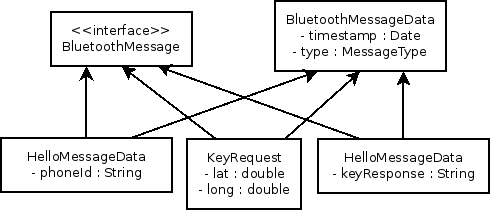
\includegraphics[scale=0.5]{resources/messages.png}}
\caption{Messages class hierarchy}
\label{img:messages}
\end{center}
\end{figure}

Using that extension of the Android \texttt{APIs} protocol messages can be easily sent using the following code:

\begin{lstlisting}[language=Java, caption=Bluetooth sending of an HelloMessage]
ObjectBluetoothSocket socket = new ObjectBluetoothSocket();
//...
BluetoothMessage msg = new HelloMessage("id", new Date());
socket.getOutputStream().write(msg);

\end{lstlisting}


\section{\textbf{Back-end}}
The back-end offers a set of \texttt{REST API} in order to authenticate the user, register a phone, upload images, audio and location. It organizes that data in a non relation database (\texttt{REDIS}) and allows to view it.\\

Images are captured and sent by Android phone in \textit{JPEG} format and are sent and displayed by the web application as they are (as shown in figure \ref{img:slideshow}).\\

\begin{figure}[!ht]
\begin{center}
\makebox[\linewidth]{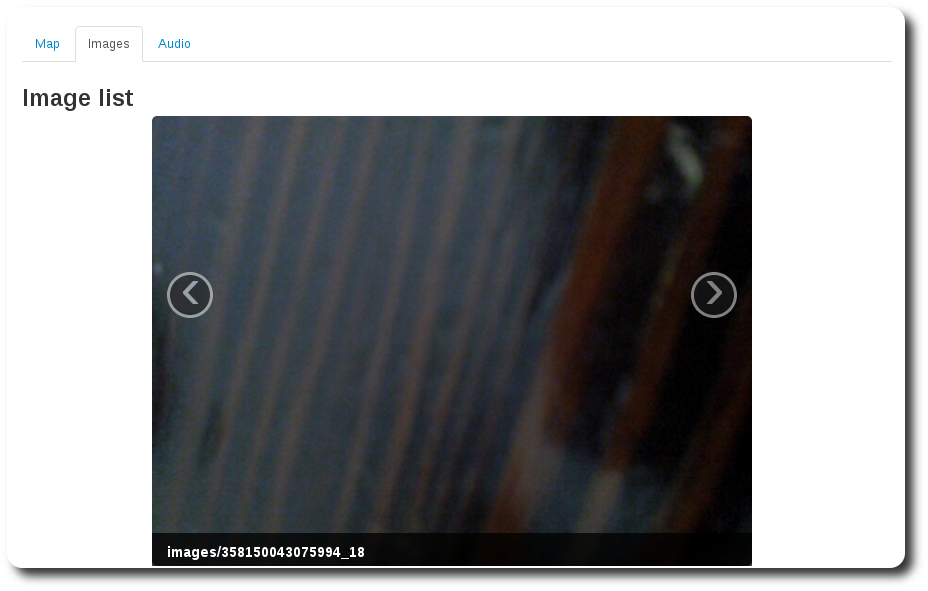
\includegraphics[scale=0.25]{resources/slideshow.png}}
\caption{Slideshow for captured images}
\label{img:slideshow}
\end{center}
\end{figure}

Audio is captured by Android phone using \texttt{AAC} encoding, unfortunately Firefox and other browsers do not support \texttt{AAC} encoding. In order to make audio available for all modern browser as soon as it is received by the web application it is converted into \texttt{vorbis} encoding using \texttt{ffmpeg}:

\begin{lstlisting}[language=Bash, caption=FFMPEG command to convert aac to mp3]
ffmpeg -i in.m4a -acodec libvorbis -aq 60 -vn -ac 2 out.ogg
\end{lstlisting}

Such a conversion is done with a background system process.\\

Uploaded location data is organized on a map created via Google Maps \texttt{APIs}.

\begin{figure}[!ht]
\begin{center}
\makebox[\linewidth]{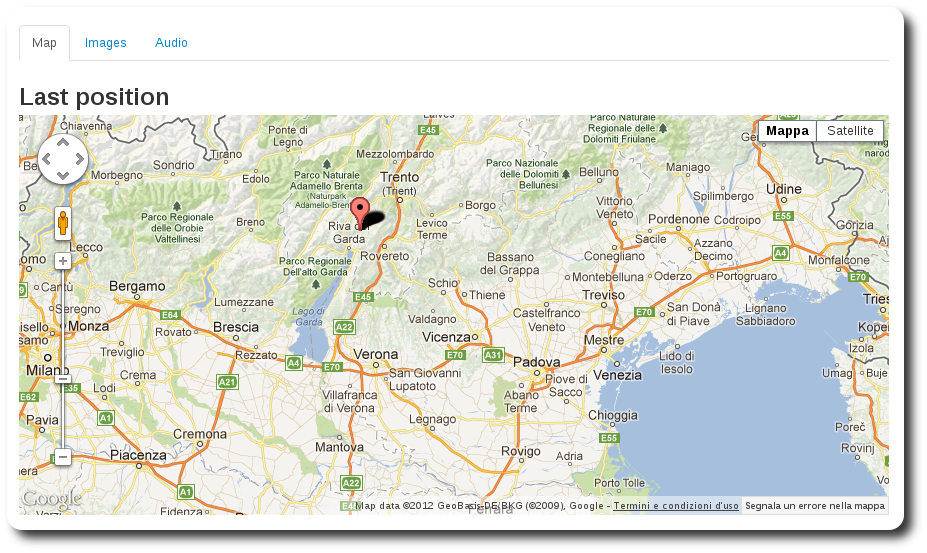
\includegraphics[scale=0.25]{resources/map.png}}
\caption{Map showing last know device position}
\label{img:slideshow}
\end{center}
\end{figure}

\section{\textbf{Related work}}
Different existing applications try to mimic a surveillance system but none of them exploits all available sensors on the phone. Moreover no phone tracking application offers a way different from direct internet connectivity to send phone's position (no opportunistic communication).\\

\begin{itemize}
	\item \textbf{Motion Detector Pro}: motion detection only app
	\item \textbf{Sound Detector}: sound detection only app. Can take pictures if the alarm is triggered
	\item \textbf{Surveillance}: motion and sound detection. Missing accelerometer motion detection, position tracking, SMS alerting and opportunistic communication
	\item \textbf{Wheres My Droid}: phone tracking app. Beta support for camera shots. Missing intrusion detection and opportunistic communication

\end{itemize}

\begin{thebibliography}{1}

\bibitem{}
B. Clifford Neuman and Theodore Ts'o (September 1994) Kerberos: An Authentication Service for Computer Networks. IEEE Communications 32. \\
\bibitem{}
S. Chita, N. Peterson, B.A. Shirazi, M. Bhadkamkar (March 2011) Home automation and security for mobile devices. PERCOM 2011. \\
\bibitem{}
I. Estevez-Ayres et al. (January 2011) Using android smartphones in a service-oriented video surveillance system. ICEE 2011. \\
\bibitem{}
Heming Pang et al. (June 2010) Research of android smart phone surveillance system. ICCDA 2010. \\
\bibitem{}
M. Mitchell (January 2011) BEAT: Bio-Environmental Android Tracking. RWS 2011. \\
\bibitem{}
G. Bianchi, P. Loreti, A. Trkulja (June 2012) Let me grab your App: Preliminary proof-of-concept design of opportunistic content augmentation. ICC 2012. \\
\bibitem{}
T. Hossmann, D. Schatzmann, P. Carta, F. Legendre (2012) Twitter in disaster mode: smart probing for opportunistic peers. MobiOpp 2012.\\


\end{thebibliography}

% that's all folks
\end{document}


